\chapter{Linkbudget}\label{ch:linkbudget}

\section{ADS-B signals}
There are currently three types of ADS-B transmissions but for satellite reception only the 1090 MHz extended squitter (ES) is of interest.  
An ADS-B message is 112 bits long and the transmission takes 120us. The modulation is Binary Pulse Position Modulation (BPPM) and the package consist of 5 parts. The first part is Downlink Format which tells that this is an ADS-B signal, second part is Additional Identifier which has different meaning within each ADS-B subtype. The third is the ICAO which is the unique identifier of the aircraft. The fourth is the DATA which contains several informations including aircraft operation status, airborne position and velocities measured from different sensors. The fifth and last is the checksum \citep{Modesorg}.      

\begin{figure}[h]
\centering 
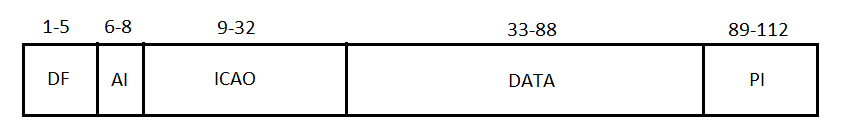
\includegraphics[scale = 0.5]{figures/adsb_signals/adsb_message.png}
\caption{112 bit long ADS-B message}
\label{fig:adsb_mes}
\end{figure}

\section{Free space loss}

Typically in satellite communication a LOS component exist. Therefore the only obstacle between the satellite and user is the atmosphere and therefore the loss can be modelled as free space, with a limited variation due to weather conditions. ADS-B signal is sent through a linear polarized monopol with power varying from 125W to 500W depending of the airplane and speed \citep{FlyingLab}. The height of a Low Earth Orbit (LEO) satellite is between 600 km to 800 km. To calculate the power loss Friis Transmission Equation is used. 

\begin{equation}
\frac{P_r}{P_t} = (\frac{\lambda}{4\pi R})^2 G_t G_r|\vec{Pr}\cdot \vec{Pt}|^2
\end{equation}

\begin{equation}
\lambda = \frac{c}{f}
\end{equation}
Where $c = 3e8$ is speed of light in vaccum and $ f$ is the frequency in Hz. $|\vec{Pr}\cdot \vec{Pt}|^2$ denotes polarization mishmash. 

\section{LEO coverage}
For a satellite the coverage area on the earth is a circular area which is defined by the height (H) of the satellite and the angel $\alpha_0$. The maximum distance the signal travels from the satellite to the earth and vice versa, is d which is depicted in figure \ref{fig:cov_sat} \citep{Cakaj2014}. The equation for d is given by equation \ref{eq:dist} 

\begin{equation}\label{eq:dist}
d=R_e(\sqrt{(\frac{H+R_e}{R_e})^2-\cos^2{\epsilon_0}}-\sin{\epsilon_0})
\end{equation}


Where

\begin{equation}\label{eq:dist2}
\epsilon_0 = \arccos{\frac{\sin{\alpha_0}(R_e+H)}{R_e}}
\end{equation}


and $R_e = 6378km$ is the radius of the earth. Further the coverage percentage of the satellite can be calculated by equation \ref{eq:coverage} which uses the total area of the earth divided by the area covered by the satellite. 

\begin{equation}\label{eq:coverage}
Coverage(\%) = \frac{A_{coverage}}{A_{earth}} = \frac{2 \pi R_e^2 ( 1 - \cos{\beta_0})}{4 \pi R_e^2}\cdot 100\%
\end{equation}
 

\begin{equation}
\beta_0 = 90 - \alpha_0 -\epsilon_0
\end{equation}


\begin{figure}[H]
\centering 
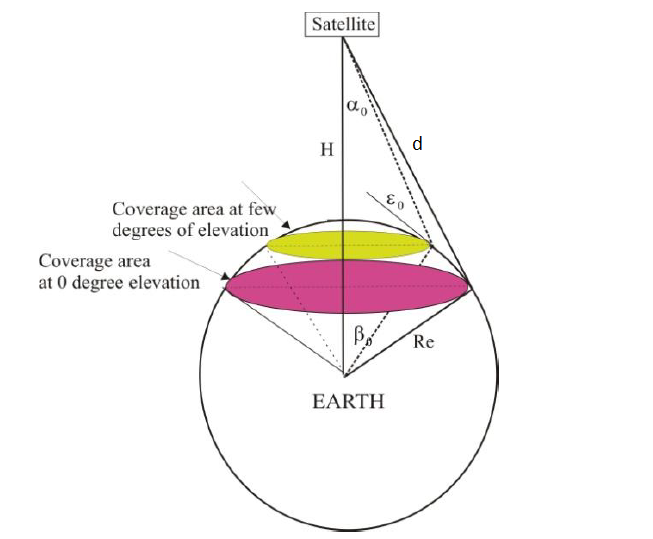
\includegraphics[scale = 0.7]{figures/linkbudget/sat_coverage.png}
\caption{Earth coverage for a satellite. Pink area is maximun coverage, green is area limited to the antenna beamwidth. \citep{Cakaj2014}}
\label{fig:cov_sat}
\end{figure} 

Because of the geometry of the earth and the height of the satellite a maximum coverage area must exist. This is depicted in figure \ref{fig:cov_sat} as purple area. To find the maximum angle of $\alpha_0$ equation \ref{eq:max_cov} is used. 

\begin{equation}\label{eq:max_cov}
\alpha_0(max) = \arcsin{\frac{R_e}{R_e+H}}
\end{equation}
 

\section{LEO radiation pattern}
Because of the unknown factor of which direction the signal arrives and which polarization the signal has, a circular polarized antenna is best suited for satellite communication \citep{Balanis2005}. Depending on the application it can ether be the ground station or satellite which polarization is circular. In this project it is desired to have the circular antenna placed at the satellite because ADS-B signals is transmitted by a linear monopole \citep{itu2017} attached to the top or bottom of the aircraft, depending of the size of the aircraft. As described earlier the signal does not always travel the same distance and therefore the loss is diffrent due to the angle of reception. The farfield of the satellite antenna should therefore compensate for this by letting the gain increase due to the angle, which is depicted in figure \ref{fig:sat_farfield}.   

\begin{figure}[H]
\centering 
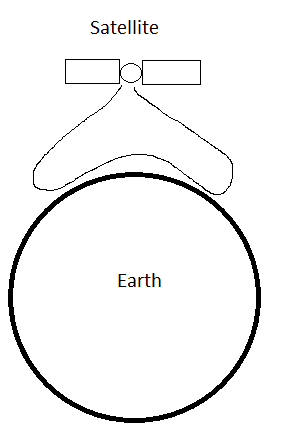
\includegraphics[scale = 0.7]{figures/linkbudget/sat_farfield.png}
\caption{Desired farfield for a LEO satellite}
\label{fig:sat_farfield}
\end{figure} 

Knowing equation \eqref{eq:dist} and \eqref{eq:dist2} a plot of the farfield can be calculated. This is done by equation \eqref{eq:coverage_farfield} where $d()$ is equation \eqref{eq:dist}. The formula normalizes the gain to an angle of zero. A plot showing the relative gain at diffrent heights is shown in figure \ref{fig:sat_farfield_plot}. It is also seen from equation \ref{eq:coverage_farfield} that the loss due to the angle is frequency independent.  
  
\begin{equation}\label{eq:coverage_farfield}
G_r(\alpha) = 10\cdot log_{10}(\frac{(\frac{\lambda}{4 \pi d(0) })^2}{(\frac{\lambda}{4 \pi d(\alpha) })^2}) = 10\cdot log_{10}(\frac{d(\alpha)^2}{d(0)^2})
\end{equation}
 

%Since the antenna is for reception the integration of the farfield should not exceed an areal of 2 to obey equation \ref{eq:farfield_cov}. 

%\begin{equation}
%2 \pi \int_0^\pi \! k \cdot G_r(\theta) \cdot sin(\theta) \, \mathrm{d}\theta = 4\pi
%\end{equation}
%\label{eq:farfield_cov}

\begin{figure}[H]
\centering 
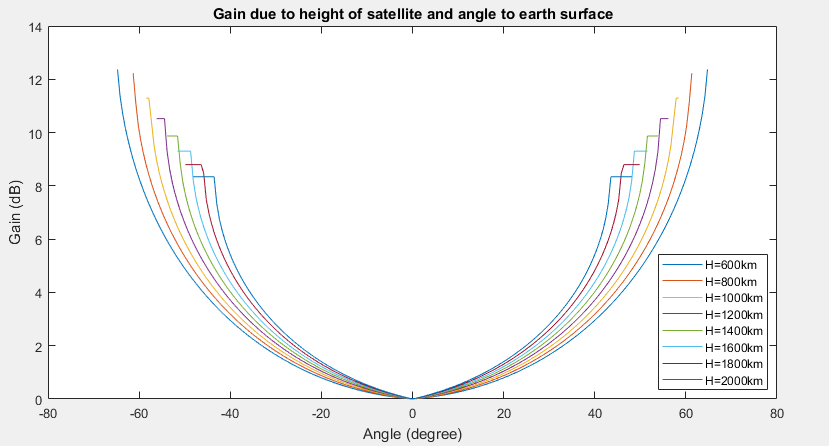
\includegraphics[scale = 0.7]{figures/linkbudget/sat_farfield_matlab.png}
\caption{Normalized gain requirement for a LEO satellite at different heights}
\label{fig:sat_farfield_plot}
\end{figure} 

\begin{center}
\captionof{table}{scaling factor} \label{tab:scaling}
  \begin{tabular}{ l  l  l  l  l}
    \hline
   \textit{Height} & \textit{Max coverage} & \textit{Max angle} \\ \hline
    600km & 3.9\%	& $64.7^\circ$   \\ \hline
    800km & 4.9\%	& $61.4^\circ$   \\ \hline
    1000km & 5.8\%	& $58.6^\circ$   \\ \hline
    1200km & 6.7\%	& $56.2^\circ$   \\ \hline
    1400km & 7.4\%	& $54.0^\circ$   \\ \hline
    1600km & 8.1\%	& $52.0^\circ$   \\ \hline
    1800km & 8.6\%	& $50.2^\circ$   \\ \hline
    2000km & 9.1\%	& $48.6^\circ$   \\ \hline
\end{tabular}
\end{center}

\section{Tabel}
With the previously description is it now easy to calculate a linkbudget. It is assumed that the receiving antenna is a circular polarized antenna which will cause a polarization mismatch at -3dB \citep{Balanis2005}. Futher an atmospheric loss at 0.1dB is assumed together with a carier to noise radio at minimum 9dB \citep{itu2017}. Loss due to cables or connectors has not been taken into account. The system noise temperature is set to 373K because of the high temperature span in the LEO \citep{FlyingLab}. The calculations is done at a transmit power at 125W and 500W which is the minimum and maximum transmit power due to the standard.   
 
\begin{center}
\captionof{table}{Linkbudget for 1090MHZ and H = 800km} \label{tab:1090}
  \begin{tabular}{ l  l  l  l  l}
    \hline
   \textit{Item} & \textit{Link parameter} & \textit{Value} & \textit{Unit} & \textit{Computation} \\ \hline
    1 & Frequency	& 1090 & MHz & \\ \hline
    2 & Transmit power (125W) & 21.0 & dB & \\ \hline
    2 & Transmit power (500W) & 27.0 & dB & \\ \hline
    3 & Transmit antenna gain & 3.0 & dBi & \\ \hline
    4 & Athmospheric absorbtion (clean air) & 0.1 & dB & \\ \hline
    5 & Free-space loss & 151.2 & dB & \\ \hline
    6 & Polarisation loss & 3.0 & dB & \\ \hline
    7 & Received carrier power & -130.3 & dB & 2+3-4-5-6\\ \hline
    8 & Bandwith (4.6MHz) & 66.6 & dB Hz & \\ \hline 
    9 & System noise temperature (373K) & 25.7 & dBK& \\ \hline 
    10 & Boltzmann's constant & -228.6 & dBW/Hz/K& \\ \hline 
    11 & Noise power & -136.3 & dBW& 8+9+10\\ \hline 
    12 & Carrier to noise ratio & 6.0 & db & 7-11\\ \hline 
    13 & C/(N+I) & 9.0 & db & Requirement\\ \hline
    14 & Antenna gain at 125W and $\alpha_0 = 0 $ & 3.0 & db & 13-12\\ \hline
    15 & Antenna gain at 125W and $\alpha_0 = \alpha_{max} $ & 15.0 & db & 14+equation \ref{eq:max_cov} \\ \hline 
    16 & Antenna gain at 500W and  $\alpha_0 = 0 $  & -3.0 & db & 13-12\\ \hline
    17 & Antenna gain at 500W and $\alpha_0 = \alpha_{max} $ & 9.0 & db & 14+equation \ref{eq:max_cov} \\ \hline \end{tabular}
\end{center}

\iffalse

\begin{center}
\captionof{table}{Linkbudget for 978MHZ and H = 800km} \label{tab:978}
  \begin{tabular}{ l  l  l  l  l}
    \hline
   \textit{Item} & \textit{Link parameter} & \textit{Value} & \textit{Unit} & \textit{Computation} \\ \hline
    1 & Frequency	& 978 & MHz & \\ \hline
    2 & Transmit power (75W) & 18.8 & dB & \\ \hline
    2 & Transmit power (500W) & 27.0 & dB & \\ \hline
    3 & Transmit antenna gain & 3 & dBi & \\ \hline
    4 & Athmospheric absorbtion (clean air) & 0.1 & dB & \\ \hline
    5 & Free-space loss & 150.3 & dB & \\ \hline
    6 & Polarisation loss & 3 & dB & \\ \hline
    7 & Received carrier power & -128.6 & dB & 2+3-4-5\\ \hline
    8 & Bandwith (4.6MHz) & 66.6 & dB Hz & \\ \hline 
    9 & System noise temperature (373K) & 25.7 & dBK& \\ \hline 
    10 & Boltzmann's constant & -228.6 & dBW/Hz/K& \\ \hline 
    11 & Noise power & -136.6 & dBW& 8+9+10\\ \hline 
    12 & Carrier to noise ratio & 8.0 & db & 7-11\\ \hline 
    13 & C/(N+I) & 9 & db & Requirement\\ \hline
    14 & Minimum receive antenna gain at $\alpha_0 = 0 $ & 1.0 & db & 13-12\\ \hline
    15 & Minimum receive antenna gain at $\alpha_0 = \alpha_{max} $ & 13.0 & db & 14+equation \ref{eq:max_cov} \\ \hline
    16 & Antenna gain at 500W and  $\alpha_0 = 0 $  & -7.23 & db & 13-12\\ \hline
    17 & Antenna gain at 500W and $\alpha_0 = \alpha_{max} $ & 4.8 & db & 14+equation \ref{eq:max_cov} \\ \hline 
  \end{tabular}
\end{center}



\begin{center}
\captionof{table}{Linkbudget for 122.5MHZ and H = 800km} \label{tab:122.5}
  \begin{tabular}{ l  l  l  l  l}
    \hline
   \textit{Item} & \textit{Link parameter} & \textit{Value} & \textit{Unit} & \textit{Computation} \\ \hline
    1 & Frequency	& 122.5 & MHz & \\ \hline
    2 & Transmit power (75W) & 18.8 & dB & \\ \hline
    3 & Transmit antenna gain & 3 & dBi & \\ \hline
    4 & Athmospheric absorbtion (clean air) & 0.1 & dB & \\ \hline
    5 & Free-space loss & 132.3 & dB & \\ \hline
    6 & Polarisation loss & 3 & dB & \\ \hline
    7 & Received carrier power & -110.6 & dB & 2+3-4-5\\ \hline
    8 & Bandwith (1MHz) & 60.0 & dB Hz & \\ \hline 
    9 & System noise temperature (373K) & 25.7 & dBK& \\ \hline 
    10 & Boltzmann's constant & -228.6 & dBW/Hz/K& \\ \hline 
    11 & Noise power & -142.9 & dBW& 8+9+10\\ \hline 
    12 & Carrier to noise ratio & 32.3 & db & 7-11\\ \hline 
    13 & C/(N+I) & 9 & db & Requirement\\ \hline
    14 & Minimum receive antenna gain at $\alpha_0 = 0 $ & -23.3 & db & 13-12\\ \hline
    15 & Minimum receive antenna gain at $\alpha_0 = \alpha_{max} $ & -11.3 & db & 14+equation \ref{eq:max_cov} \\ \hline
  \end{tabular}
\end{center}

\fi